\subsection{Entstehung der Idee}

In Städten wie London oder Wien ist dem Projektbetreuer aufgefallen, dass immer mehr Stadtbewohner Fahrräder nutzen, es aber große Defizite bei sicheren Abstellplätzen gibt. Zuhause werden teure Fahrräder nicht selten auf die kleinen, wertvollen Balkone der Privatwohnungen (sicher) abgestellt. Einmal mit dem Fahrrad im stadtzentrum, wird es noch schwieriger. Das Projektteam vertritt die Hypothese, dass viele Stadtbewohner auf das Fahrrad umsteigen werden, sobald dieses Problem zufriedenstellen gelöst ist. Daraus formte sich die Idee eines „Fahrradturms“. Wie der Name schon verrät, ist ein Fahrradturm eine turmförmige Konstruktion, in der möglichst viele Fahrräder auf kleinstem Raum gelagert werden können. Die Vision sieht vor, die Fahrräder mittels automatischer Lagerroboter auf mehrere vertikalen Ebenen aufzuteilen, um die Platzeffizienz weiter zu steigern.

\begin{figure}[H]
  \begin{center}
    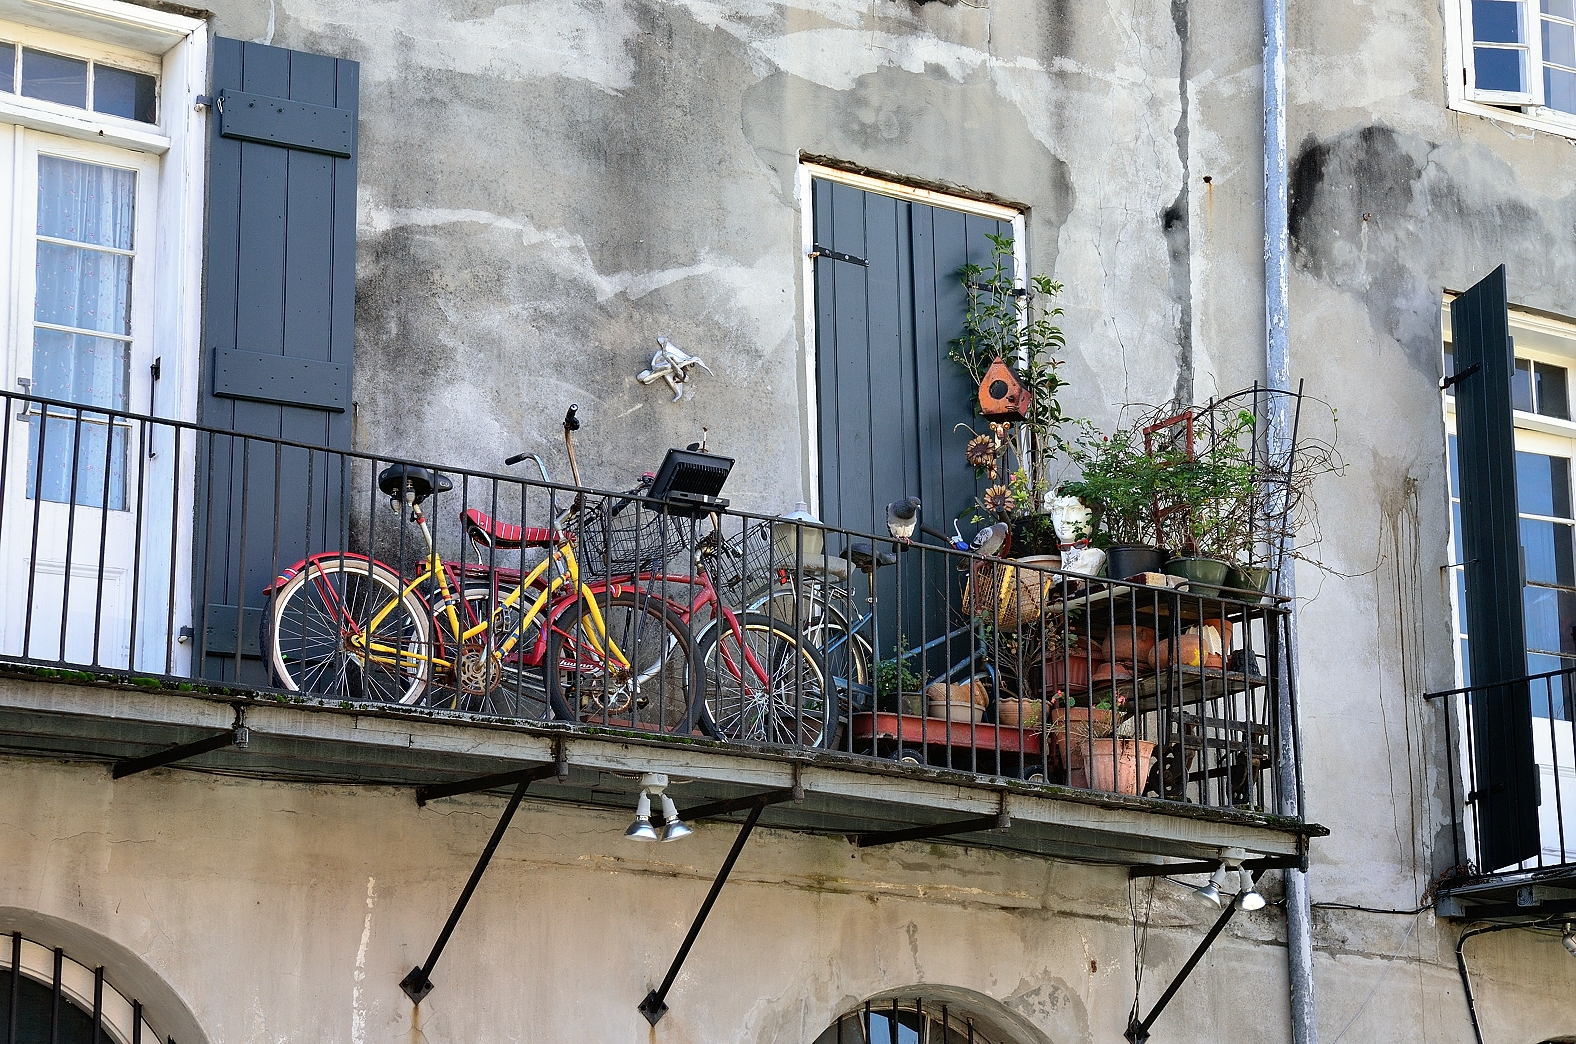
\includegraphics[width=0.5\textwidth]{images/fahrrad_balkon.jpg}
    \caption{Fahrrad auf Balkon\cite{fahrrad_balkon}}
    \label{fig:fahrrad_balkon}
  \end{center}
\end{figure}